\documentclass[12pt,a4paper]{article}
\usepackage[utf8]{inputenc}
\usepackage[T1]{fontenc}
\usepackage[italian]{babel}
\usepackage[margin=2cm]{geometry}
\usepackage{graphicx}
\usepackage{float}
\usepackage{url}
\usepackage[breaklinks=true]{hyperref}
\usepackage{xurl}

% Definizione del comando pandocbounded per le immagini
\providecommand{\pandocbounded}[1]{#1}

% Definizione del comando tightlist (usato da Pandoc)
\providecommand{\tightlist}{%
  \setlength{\itemsep}{0pt}\setlength{\parskip}{0pt}}

\title{Aggiornamenti sul progetto per la simulazione di reti veicolari con comunicazione satellitare tramite 5G}
\author{}
\date{}

\begin{document}
\maketitle

\section{Adattamento del modulo ns-3 leo}\label{adattamento-del-modulo-ns-3-leo}

Come base per l'implementazione del sistema satellitare è stato utilizzato il progetto ns-3-leo~\cite{ns3leo}\cite{ns3leoarticle}, che tuttavia presenta le seguenti limitazioni:

\begin{itemize}
\tightlist
\item
  Risulta obsoleto e non compatibile con le ultime versioni di ns-3
\item
  Manca di alcune funzionalità (movimento di oggetti terrestri a velocità costante)
\end{itemize}

Il lavoro svolto ha quindi comportato:

\begin{itemize}
\item
  Migrazione del sistema di build da wscript a CMake per garantire la compatibilità con le versioni più recenti di ns-3
\item
  Risoluzione di numerosi bug e problemi di compilazione che impedivano l'utilizzo del modulo con clang (compilatore più rigoroso riguardo alla sintassi C++ e al controllo dei tipi, ad esempio l'uso di 0 o NULL invece di nullptr, incongruenze di tipi)
\item
  Aggiornamento delle funzioni interne per garantire la compatibilità con i moduli più recenti
\item
  Integrazione di ns-3-leo con il modulo nr (5G-LENA~\cite{5glena}) sull'ultima versione di ns-3
\item
  Implementazione di un nuovo mobility model che consente di modellare il movimento a velocità costante di un oggetto da una posizione specifica (longitudine, latitudine, altezza) verso una direzione definita (specificando l'azimut) sulla superficie terrestre, idealizzando la forma del globo come una sfera semplice
\end{itemize}

Il nuovo mobility model è stato sviluppato utilizzando come riferimento il ground model già presente per le stazioni fisse~\cite{ns3leo_groundhelper} e, principalmente, il mobility model del satellite~\cite{ns3leo_mobility}. Sebbene quest'ultimo presentasse logiche simili, il suo modello di movimento era strettamente legato alle orbite, rendendo necessaria una riscrittura sostanziale delle funzioni e delle formule che modellano il movimento.

\begin{itemize}
\tightlist
\item
  Implementazione di un esempio per il tracciamento dei movimenti del nodo veicolo sulla superficie terrestre a velocità costante e di un satellite, con output delle coordinate istantanee
\end{itemize}

Il mobility model è stato sviluppato partendo dall'esempio di tracciamento orbitale circolare~\cite{ns3leo_example} e successivamente adattato allo scenario richiesto.

\begin{itemize}
\tightlist
\item
  Sviluppo di uno script Python per la visualizzazione tridimensionale dei punti elaborati dall'esempio precedente, utilizzando matplotlib per la rappresentazione grafica dei risultati (come mostrato in Figura~\ref{fig:car_move_model})
\end{itemize}

\begin{figure}[H]
    \centering
    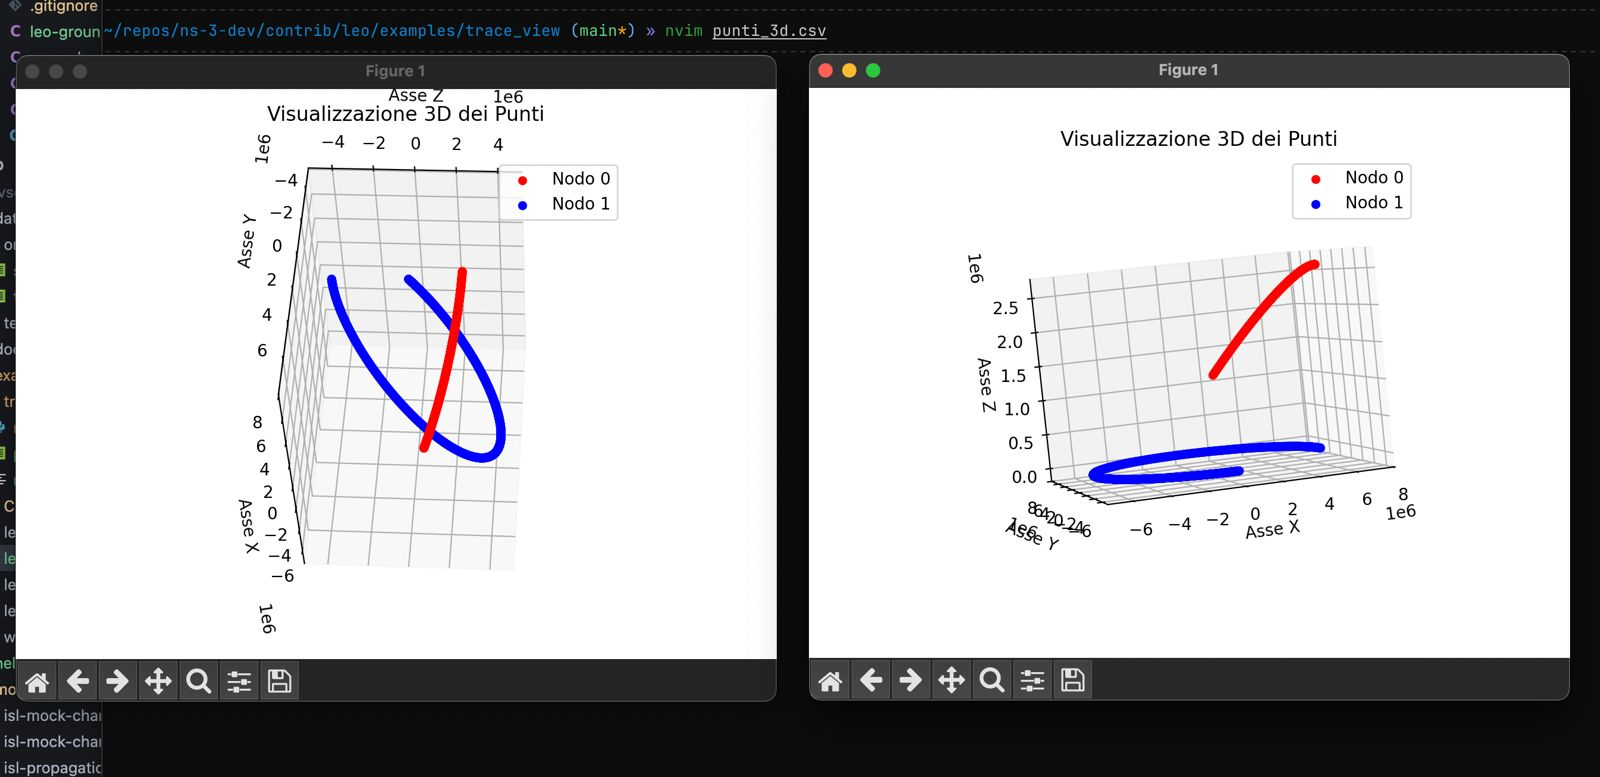
\includegraphics[width=0.8\textwidth]{assets/move-model.jpg}
    \caption{Move Model Graph Examples}\label{fig:car_move_model}
\end{figure}

\begin{itemize}
\tightlist
\item
  Fork del progetto epidemic-routing per garantire la compilabilità di tutti gli esempi già presenti in ns-3-leo, adottando anche in questo modulo il sistema di build CMake
\end{itemize}

\textbf{Note tecniche:}

Il modulo ns-3-leo utilizza orbite sferiche semplificate che non tengono conto di fattori aggiuntivi e non sono ellittiche. Il sistema costruisce un pianeta sferico al centro delle coordinate e posiziona i satelliti su diverse orbite (i cui piani orbitali richiederebbero ulteriori chiarimenti), distribuendoli equidistantemente e facendoli muovere a una velocità calcolata in base all'altitudine su orbite circolari nella direzione prevista.

In alternativa, il progetto Hypatia~\cite{hypatia} utilizza ns3-satellite~\cite{ns3satellite} come modulo per il movimento satellitare, implementando il modello SGP4/SDP4 (modello americano che offre previsioni più accurate). Sebbene sia possibile considerare l'adozione di questo modello in sostituzione a quello di ns-3-leo, l'approssimazione attualmente utilizzata potrebbe risultare sufficiente per i casi d'uso specifici del progetto.

\textbf{Risorse utili:} Dataset satelliti Starlink~\cite{starlink_dataset}

\section{Implementazione della comunicazione satellite-veicolo con 5G-LENA}\label{inizio-di-implementazione-della-comunicazione-satellite-veicolo-con-5g-lena}

\begin{itemize}
\tightlist
\item
  Sviluppo di un esempio in ns-3-leo basato sull'esempio CTTC 3GPP~\cite{cttc_3gpp_example} e sulla simulazione precedente per testare la comunicazione 5G-LENA~\cite{5glena} tra un satellite e un veicolo terrestre, utilizzando il mobility model precedentemente implementato.
\item
  Reimplementazione del visualizzatore utilizzando Plotly per il rendering 3D con accelerazione GPU, consentendo la visualizzazione dei dati di movimento di satellite e veicolo e il debugging del mobility model e della comunicazione. Il sistema offre un'interfaccia interattiva per visualizzare latitudine, longitudine e altezza di satellite e veicolo, nonché le loro posizioni nello spazio tridimensionale (Figura~\ref{fig:new_vis_trace_orbits}).
\end{itemize}


\begin{figure}[H]
    \centering
    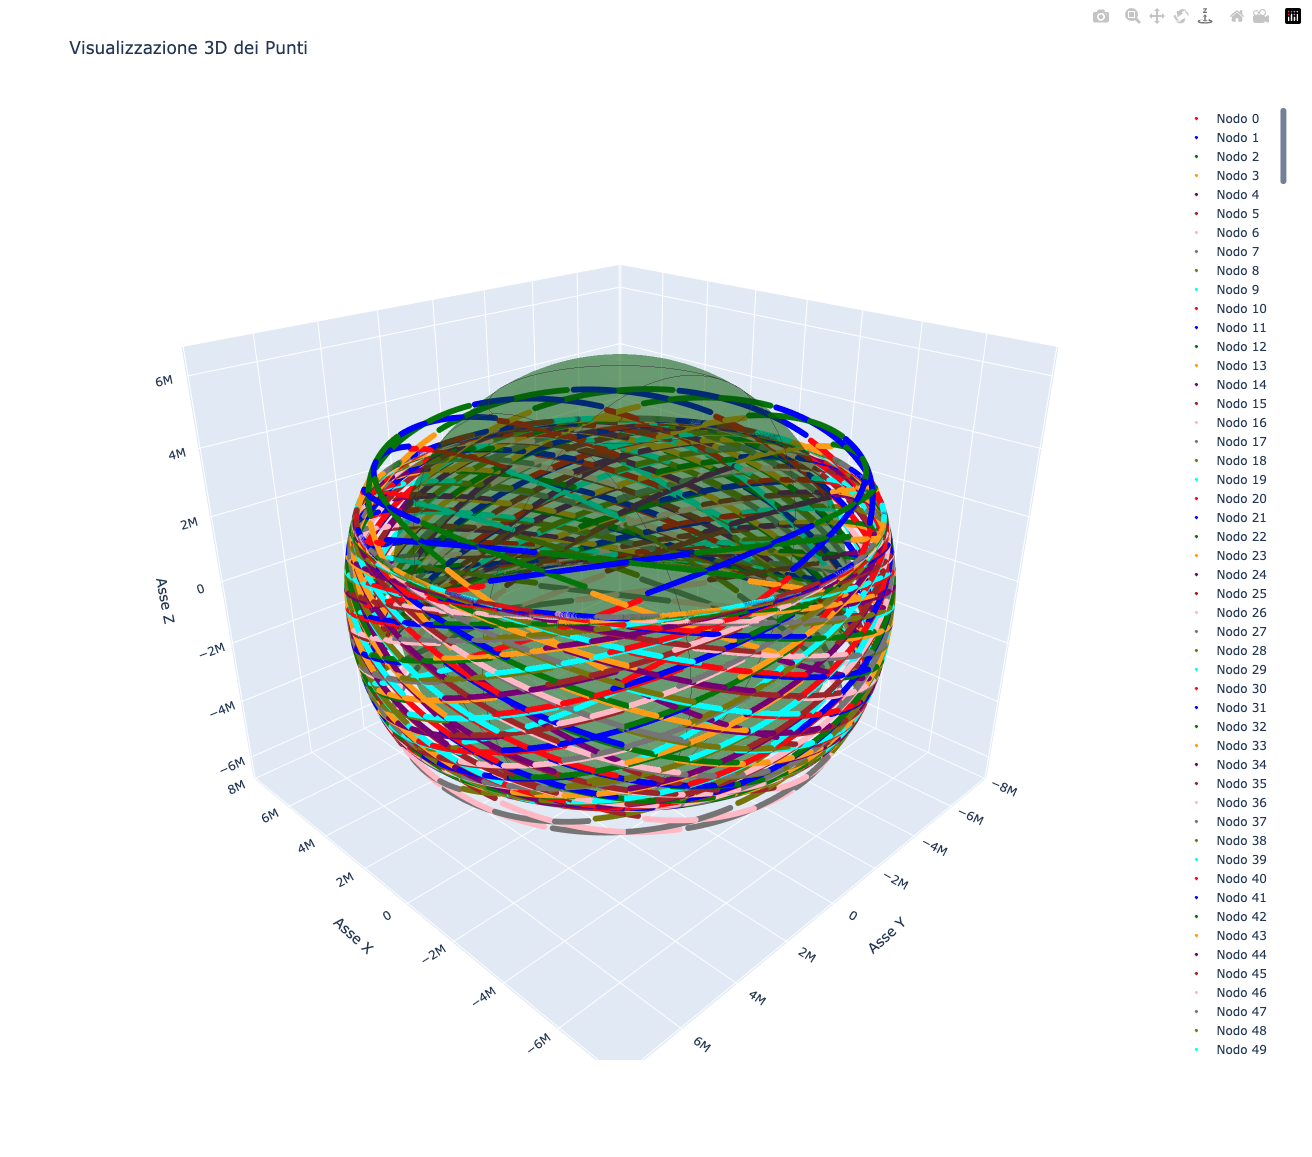
\includegraphics[width=0.8\textwidth]{assets/new_vis_trace_orbits.png}
    \caption{Orbits tracing with plotly with interactive interface GPU accelerated}\label{fig:new_vis_trace_orbits}
\end{figure}

\begin{itemize}
\tightlist
\item
  Integrazione con i modelli NTN (Non-Terrestrial Networks) di ns-3: rimodulazione dei Mobility Model per supportare le coordinate geocentriche, necessarie per l'utilizzo degli scenari NTN e per l'implementazione dei modelli di propagation loss 3GPP. L'implementazione è stata realizzata derivando il mobility model GeocentricConstantPositionMobilityModel~\cite{ns3_ntn_workshop}, poiché i controlli interni di ns-3 vengono effettuati esclusivamente su questa classe (non esistendo una classe virtuale per questi modelli), come evidenziato nel codice sorgente~\cite{ns3_channel_condition} alla riga 585. È importante notare che i metodi utilizzati per l'impostazione della posizione non sono completamente funzionali e richiederebbero l'implementazione di un MobilityHelper personalizzato che utilizzi i setter della posizione tramite coordinate geocentriche anziché topocentriche (coordinate standard).
\item
  Utilizzo degli esempi NTN~\cite{ns3_ntn_example} e CTTC 3GPP~\cite{cttc_3gpp_example} per la realizzazione di uno scenario con un'automobile e un satellite in comunicazione tramite 5G-LENA~\cite{5glena}, utilizzando i mobility model precedentemente creati e il propagation loss model ThreeGppPropagationLossModel in ambiente suburbano (configurabile).
\item
  Implementazione nel LeoOrbitNodeHelper della possibilità di specificare la precisione del modello di movimento, consentendo l'aggiornamento della posizione del nodo con frequenza personalizzabile (ad esempio ogni 50ms) invece del default di un secondo.
\item
  Implementazione dei metodi per il calcolo del SNR tra satellite e veicolo, basati sugli esempi precedentemente citati, utilizzando le antenne dei dispositivi e il propagation loss model 3GPP per determinare la qualità del segnale tra i nodi.
\item
  Integrazione nell'esempio di comunicazione NR di estesi output di debug per le condizioni di rete e lo stato della comunicazione, collegando il gNB satellitare tramite canale Point-to-Point a un nodo di rete dedicato alla risoluzione delle problematiche di configurazione di 5G-LENA~\cite{5glena}, permettendo il successo della comunicazione UDP tra satellite e veicolo. Lo scenario implementato è illustrato in Figura~\ref{fig:initial_nr_scenario_sim}.
\item
  Ristrutturazione della gestione del parametro ``precision'' e dello scheduling degli aggiornamenti di posizione per nodi veicolo e satellite, risolvendo bug di sincronizzazione e migliorando la stabilità del sistema, evitando scheduling di eventi non necessari.
\end{itemize}

\begin{figure}[H]
    \centering
    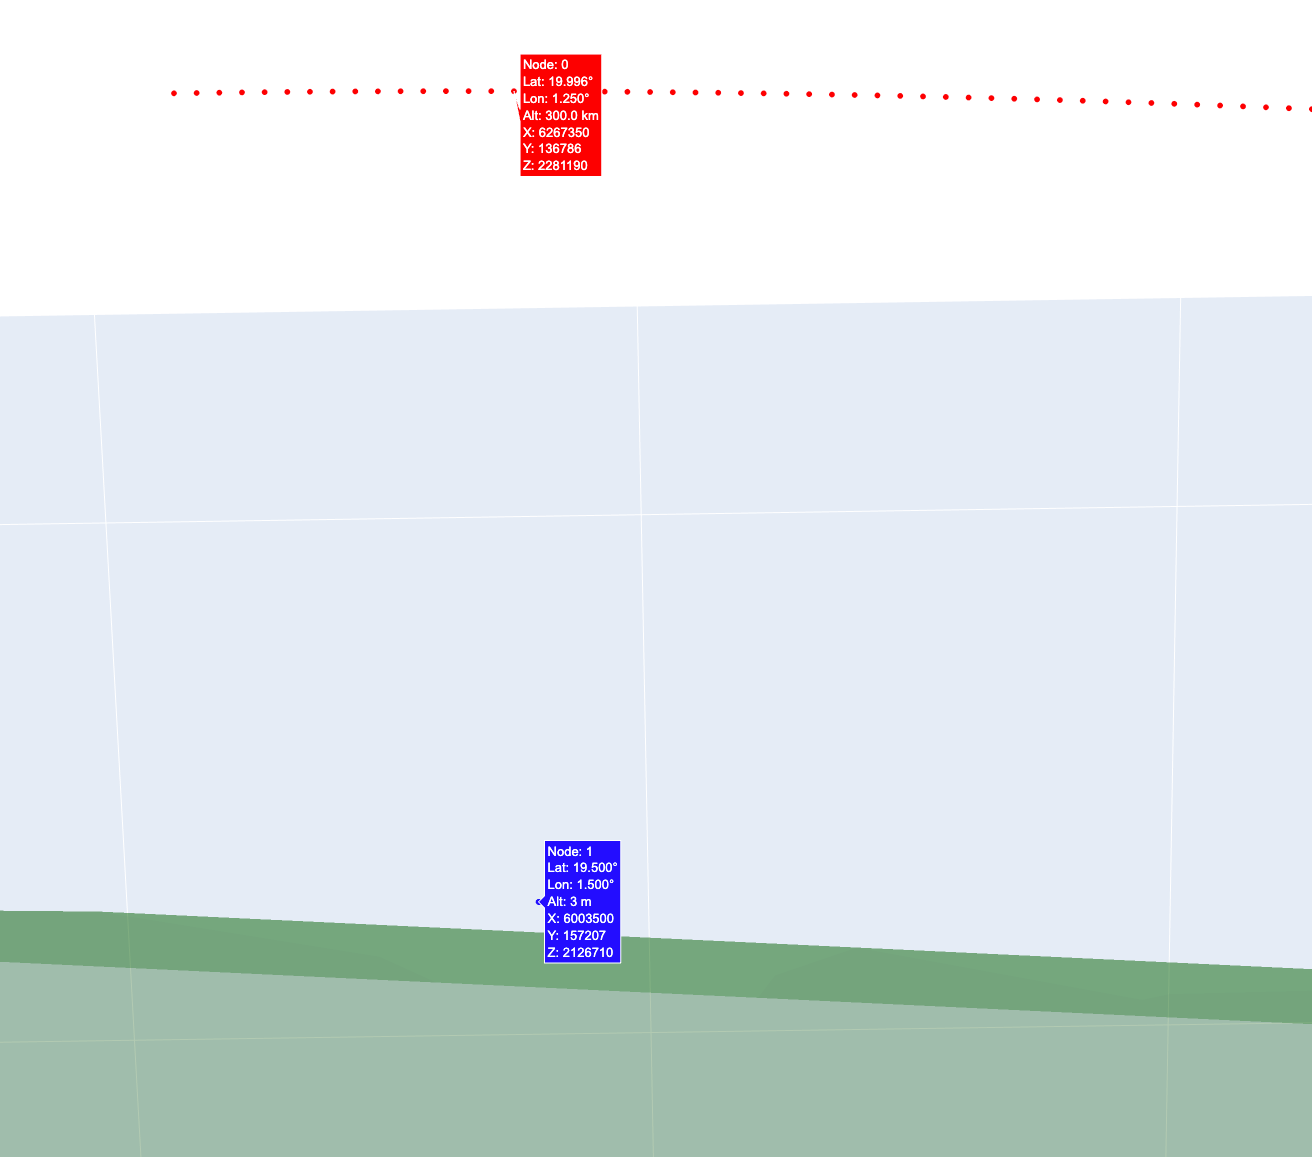
\includegraphics[width=0.5\textwidth]{assets/satellite_and_car_nr_simulation.png}
    \caption{Simulation Scenario with 1 car and 1 satellite communicating with 5g-lena}\label{fig:initial_nr_scenario_sim}
\end{figure}

\bibliographystyle{unsrt}
\phantomsection{}
\addcontentsline{toc}{section}{Bibliografia}
\bibliography{bibliografia}

\end{document}
